\documentclass[12pt]{article}

% preamble begins
\title{CS261 Final Report}
\author{Team 29 \\\\ \textbf{Sylvester Cardorelle},\textbf{Tudor Cismarescu}, \textbf{Ollie Madelin},\\
\textbf{Josh Footman}, \textbf{Joseph Parkins}, \textbf{Anil Kiral}}
\date{March 2017}
\usepackage{graphicx}
\usepackage{listings}
\usepackage{scrextend}
\usepackage{titlesec}
\usepackage{float}
\usepackage[margin=1.2in]{geometry}
%preamble ends


%content begins
\begin{document}
\begin{titlepage}
\maketitle
\centering
\vfill
\vfill

\includegraphics[width=7cm]{logo.png}
\vfill
\vfill
\thispagestyle{empty}
\end{titlepage}
\tableofcontents
\section{Installation Guide/ System Requirements}
	\subsection{Setup}
		\subsubsection{Node}
    \subsubsection{SQL}
    \subsubsection{Angular}
    \subsubsection{Npm Installation}
  \subsection{Running}
\section{User Guide}
  \subsection{Analysis tab}
  \subsection{Live Stream tab}
  \subsection{Historical Data tab}
\section{FAQs}
\section{Research}
  After the analysis and design of the project, our software development team had developed a stronger idea
  of the technologies that would be used to design the system. This section further expands on the decisions and
  research that was made after the first deliverable that allowed us to finalise our choice of technologies.
  \subsection{Front-end}
  The \textbf{AngularJS} framework was used to build the frontend as planned. We considered other JavaScript frameworks,
  such as \textbf{React}, however we felt that Angular was the better choice being a full-fledged MVC (Model-View-Controller) framework,
  which has been in use for a much longer time than other JavaScript frameworks, thus boasting a detailed documentation and various fully-tested features.
  As our system is essentialy a single page application (SPA) which will update dynamically, AngularJS became a natural choice for our developers.
  \newline
  After this decision was made between the PM and Developers, our front-end developers took the initiative to intensively learn AngularJS using a multitude online resources.
  For example, Codecademy a programming teaching platform was used to learn Angular basics, whilst Angular Community pages were used to further expand their knowledge.
  \subsubsection{Graph Libraries}
  - Chart JS
    - responsive
    - sparse documentation
    - only supports 6 basic chart types
  - Plotly JS
    - used for financial graphs , well supported graph types e.g. candlestick graphs etc.
    - can export generated graph as png for further inspection
    - can zoom into generated graph and scrutinise specific areas
    - can save graph directly onto a cloud platform
  \subsection{Back-end}
    \subsubsection{Server-Side Script}
    Django (Python) - no one in group was familiar , decided not to use python due to time restrictions
    Ruby on Rails(Ruby) - same as above
    Express (Node.JS) - minimalist , built on our exisiting skills of JavaScript
    Java was carried forward for the data analysis
    \subsubsection{Database}
    -decided between MySQL and SQLlite
      - however backend developers preferred to leave out database from the systems implementation
      this is because to avoid the bottleneck of querying data from the database rather than
      caching the data with Java abstract data structures and storing a data for a certain amount
      of time then storing historical data within the database that would not be useful in further
      algorithmic calculations
\section{Design}
  \subsection{User Interface}
    - color scheme
    - font size
    - abstraction
      - simplicity
         we wanted to develop something that did not require a manual essentialy,
         the apps fundamental operation can be grasped by the client with the assumption
         that they are computer literate.
  \subsection{Pseudocode}
    This section explores the type of algorithms that we used to analyse the input stream of data for anomalies.
    \subsubsection{Pump \& Dump}
    Arguably, Pump \& Dump was the most challenging type of price manipulation that we attempted to detect.
    After researching the characteristics of a Pump \& Dump, our team concluded the following about Pump \& Dump:
    \begin{itemize}
      \item A large batch of cancellation orders before the dumping of stocks by a person or group (\textbf{Non-Detectable with current data set})
      \item A steady increase of stocks value from the average value, when the Pumping begins (\textbf{Detectable})
      \item A sudden drop in price when the dumping of stocks occur (\textbf{Detectable})
    \end{itemize}
    PICTURE OF PUMP DUMP EXAMPLE HERE
    By identifying the traits of a Pump \& Dump, we were able to construct pseudocode that would later be transformed
    into Java code.
    \begin{figure}[H]
    \centering
    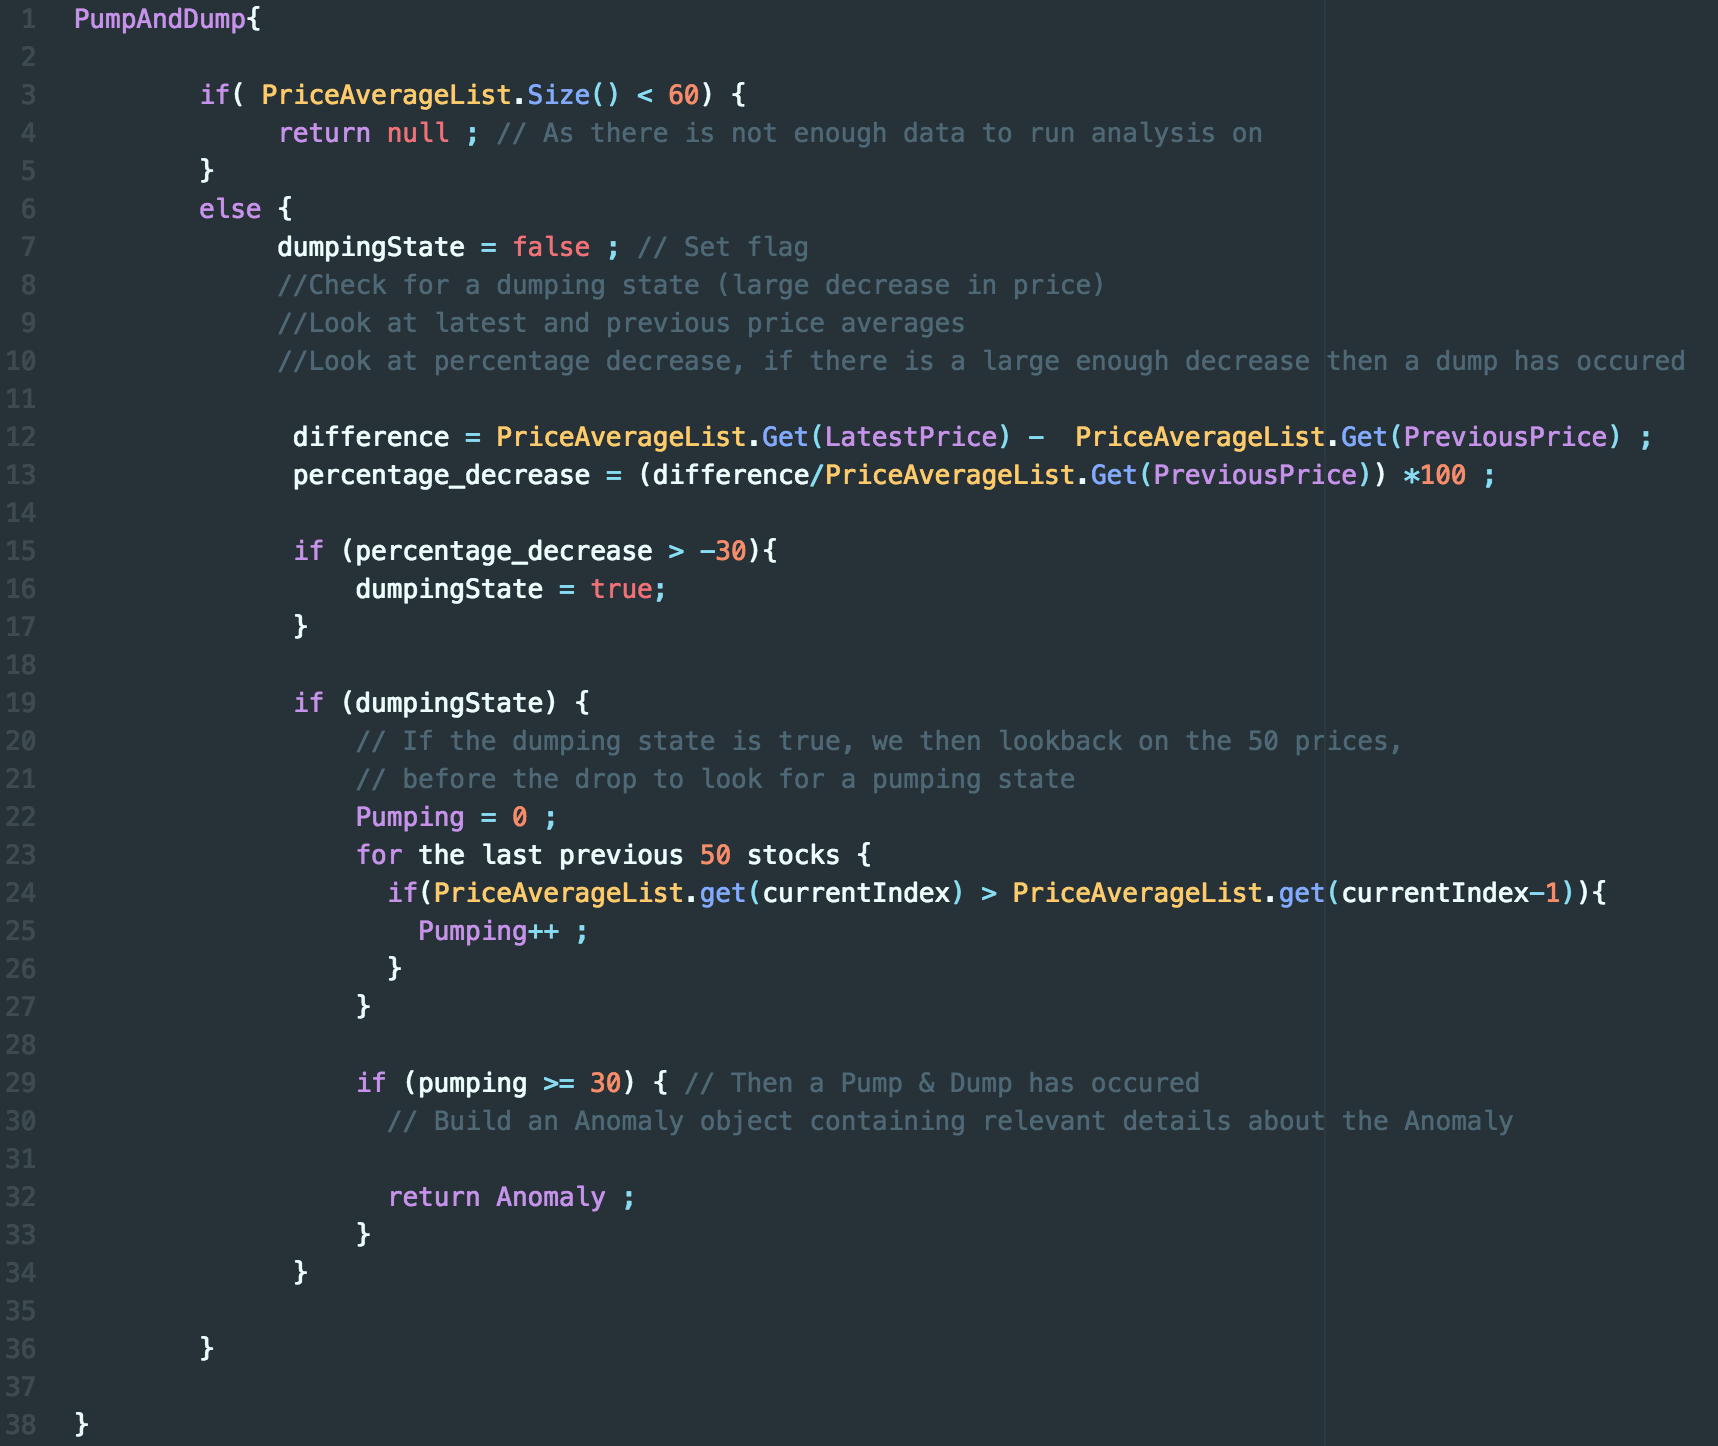
\includegraphics[width=150mm]{PDpseudo.png}
    \caption{Pump \& Dump Pseudocode}
    \end{figure}

    \subsubsection{Volume Spike}
    \subsubsection{Fat Finger Errors}
\newpage
\section{Implementation}
  \subsection{Frontend}
  \subsection{Backend}
    \subsubsection{Parsing}
\section{Iterations}
  \subsection{Iteration 1}
  \subsection{Iteration 2}
  \subsection{Iteration 3}
  \subsection{Iteration 4}
  \subsection{Iteration 5}
\section{Testing}
  \subsection{Unit Testing}
    \subsubsection{Angular Dependency Injection}
  \subsection{Integration Testing}
  \subsection{System Testing}
  \subsection{User Acceptance Testing}
    \subsubsection{Email Correspondence}
\section{Project Management}
  \subsection{Overview}
  \subsection{Roles}
\section{Evaluation}
\end{document}
% Content ends
